\documentclass[UTF8]{ctexart}

% \usepackage{authblk} % 作者信息
\usepackage[super]{gbt7714} % 国标 - 引用
\usepackage[colorlinks, linkcolor=blue, anchorcolor=blue, citecolor=green]{hyperref} % 超链接

\usepackage[raggedright]{titlesec}% 设置每节的标题居左显示

\usepackage{lastpage}

\usepackage{graphicx} % 图片相关
\usepackage{float}

\usepackage{fancyhdr} % 清除之前页眉页脚的设置
\pagestyle{fancy}
\renewcommand\footrulewidth{0pt}


\usepackage{mathrsfs} % 数学问题
\fancyfoot[C]{\thepage} % 页脚中间显示页码

%\usepackage{geometry} % 边距设置
%\geometry{a4paper, scale=0.85}

\begin{document}

\title{基于电生理学的多通道猪只应激水平监测}
\author{}
\date{\today}

\maketitle
\thispagestyle{empty}

% --- 目录 ---

\newpage
\pagenumbering{roman} % 用罗马数字计数
\fancyhead{} % 不显示页眉
\tableofcontents

% --- 正文 ---

\newpage
% 页眉设置
\lhead{第 \thepage\ 页,共 \pageref{LastPage}\ 页} % LaTeX -> LaTeX
\rhead{}%\small\leftmark}
\setcounter{page}{1}   % 从这里开始计数
\pagenumbering{arabic} % 采用阿拉伯数字计数

\section*{更新历史}

\begin{itemize}
    \item 2022-05-16 ~初始文档
    \item 2022-05-17 ~确定人选,第一次提交
    \item 2022-05-21 ~微小改动,使行文更加顺畅
    \item 2022-05-22 ~修改标题以及行文,添加超链接
    \item 2022-05-24 ~规范化格式,修改口语化的内容
    \item 2022-05-27 ~根据实际进度添加图片以填充细节
\end{itemize}

\newpage
\section{团队介绍}

参赛成员总共有4人,来自两个不同的专业。其中两人来自动物科学专业,两人来自电子信息科学与技术专业,属于
跨学科合作,而我们的选题以及解决方案也正需要不同学科交叉融合的努力才能产生成果。
\par
下面简单介绍参与的人员以及主要任务(考虑到隐私抹去名字):
\begin{itemize}
    \item GES,\emph{队长}
    \begin{itemize}
        \item AS专业,主要负责框架的设计以及Web服务的实现
    \end{itemize}
    \item LYH,\emph{队员}
    \begin{itemize}
        \item AS专业,主要负责检测预警模型的设计、实现以及调参
    \end{itemize}
    \item ZXG,\emph{队员}
    \begin{itemize}
        \item EE,主要负责传感器以及放大电路的设计
    \end{itemize}
    \item ZZY,\emph{队员}
    \begin{itemize}
        \item EE,主要负责设备的无线传输功能以及数据的预处理
    \end{itemize}
\end{itemize}

\newpage
\section{关于课题}

我们选择的方向是「猪行为监测方法」。

\subsection{任务分析}

监测行为的最终目的之一就是观察动物的状态,考虑到时间成本以及技术力,
我们放弃了对动物的动作进行探测而选择直接选择监测生理状态,使用传感器所采集的生理数据(我们的想法是采集
皮肤电活动以及表情肌活动等电生理数据)来进行\textbf{实时}以及\textbf{连续}的应激程度分析
以及预警。因此对项目而言:
\par
\textbf{输入}是家畜的生理数据 \footnote{我们计划采集皮肤电活动与表情肌活动。};
\par
\textbf{输出}是应激程度或压力水平。

\subsection{Overview}\label{sec:22}

详见下面的图 \ref{fig:flowchart} :

\begin{figure}[H]
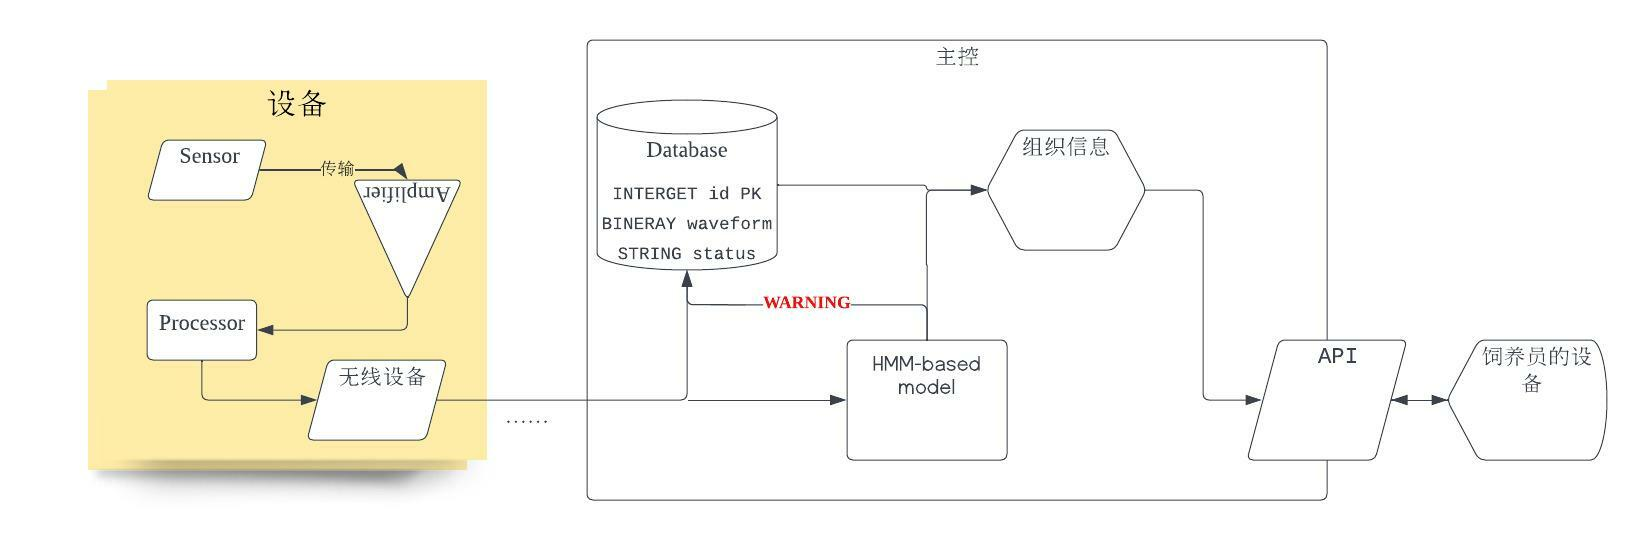
\includegraphics[width=0.95\textwidth]{fc.jpeg} % 可能需要一些改变 不,就这样吧
\centering
\caption{系统运行的大致流程}
\label{fig:flowchart}
\end{figure}

不难看出,我们把整个监测系统分成了以下几个部分:

\begin{itemize}
    \item 传感器
    \item 主控
    \item 终端
\end{itemize}

通过较小的、可以粘附在猪身上而不对其造成太大影响的传感器,将皮肤导电程度以及其变化
传输到监测单元(主控)进行分析,实时检测并且将结果以及原始数据持久化保存,如果
检测到存在应激的情况,将自动报警并且返回个体的标识以及异常的生理数据本身。
\par
其中,监测单元可以架设在养殖场的某台设备上,也可以上传至云端与
多组数据\footnote{例如采食量、精液品质、胎次、日增重等等。}进行联合检测以及整合分析。

\section{解决方案}

\subsection{引言}\label{sec:31}

随着畜牧集约化的发展,对家畜的生产性能要求逐步提高,\textbf{应激}这一消极现象以及其引发的后果也得到了重视。
但是很多对应激的测量方式要么无法持续的实时检测,要么对家畜有所损害,测量应激的过程本身也导致了应激,所以\textbf{无损检测}这一概念因此出现。
无损监测是指在不损害或不影响被监测对象的前提下,借助现代技术和设备对监测对象内部及表面的结构、性质、状态等进行监控和测试的方法。
而畜牧业的无损检测就是在不损害或不影响的前提下对家畜进行检测。\cite{wang2017monitor}
而我们需要获取行为相关数据的目的,就是针对目标的情绪(主要是愉悦以及应激)进行分析,这就涉及了\textbf{情感计算}。
\par
按照维基百科的定义,情感计算属于一类跨学科的领域,旨在研发能够识别、解释、处理、模拟情感的系统。
在1995年,Picard 的文章 Affective Computing\cite{picard1995ac}的发表标志着这个领域的正式诞生。
而随着知识的积累以及技术的发展,对情感,或情绪的描述也逐渐的丰富,产生了一系列模型,主要包括了\textbf{分类模型}以及\textbf{连续模型}两类。
其中,前者是针对表情做出了简单的,诸如「高兴」、「悲伤」、「恐惧」等的分类;
而后者是将感情看作在一系列的维度组成的空间下的向量。其中,就检测方式来讲,检测模型包括文字检测、语音检测以及表情检测等等。
\par
但关于动物的情感分析,就更加少之又少,不过随着人们对动物福利意识的提高、对动物的情绪对生产性能的影响的认识逐渐深刻\cite{wang2017monitor},
针对动物的情感分析的研究方向也有了一些进展,Anil等\cite{anil2006pain}以猪为实验对象,通过行为以及若干生理参数,来对猪的痛感这种消极情绪体验进行研究;
来自荷兰瓦赫宁根大学动物科学系的 Neethirajan 等人\cite{neethirajan2021happy},基于Yolo(一种目标检测模型)以及RCNN(一种特殊的卷积神经网络),
采用深度学习算法针对家畜的面部的一系列特征设计了一套算法,可以检测动物的表情以及表情反应的情绪。
\par
动物的压力水平很容易通过神经系统对汗腺的刺激以皮肤微小的排汗量的变化再以皮肤的导电程度来体现,这个反应被称作\textbf{皮肤电反应}(\emph{galvanic skin response, GSR})。
而猪的身体鲜有具有排汗功能的汗腺,主要是位于肢体、职责是释放外激素且难以检测到排汗量的腕腺(gll. carpeae)\cite{raghav1comparative}
以及位于鼻镜上具有排汗功能的鼻镜腺,其中基于组织学以及免疫学方法的研究证实了牛的鼻唇腺受副交感神经调控\cite{ceccarelli1986innervation}。
但是另一个采用电镜进行物种鉴定的研究中,猪的鼻镜腺开口数目不算很大\cite{madkour2022scanning},这也为项目的研究以及落地带来了挑战。
\par
在上文 Neethirajan 的研究中,他们通过设计确定了采用特定的表情特征(例如耳朵被抬起的高度、暴露的眼白面积等等)作为判定情绪的依据,
而研究后文的结果显示该方法取得了不错的效果,所以采取表面肌电图(\emph{surface electromyography, sEMG})设备对动物的表情肌进行采样以获取情绪或应激程度也是可行的。
动物很少隐藏情绪,因此从对表情进行分析也可以取得不错的成果。
\par
在针对动物的肌电图的研究很少,但是针对人的无论是研究还是成果都很多,而同属动物无论是从微观还是宏观上具有相似的构造以及性质,
因此将用于人的 sEMG 系统迁移并移植到动物作为连续工作的情绪监测系统也是可行的。

\subsection{方案论述}

如上文第 \ref{sec:22} 节中所示,我们的思路就是对家畜的应激程度或是压力水平做出定量的测定,
因此我们需要一个能够反应动物应激水平的测量方法,这种方法需要存在着以下的性质:

\begin{itemize}
    \item该器官/组织能够受神经作用,能够反映某种神经活动
    \item受神经调控的变化能够被轻易观测到
    \item其他环境因素对其的\textbf{直接}影响不大\footnote{拿人类的排汗以及心率为例,排汗受神经系统的\textbf{直接调控}而心率不仅仅受神经系统的调控。}
\end{itemize}

启发我们的想法就是针对人类的姿势分析、骨骼提取以及后续分析的相关研究成果以及产品(详见前文第 \ref{sec:31} 节),
可以很轻易地联想到躯体战栗或强直代表着紧张。因此我们最开始的想法是针对猪或鸡的姿势进行分析。
\par
但是因为单纯的\textbf{姿势估计}(\emph{pose estimate})以及\textbf{动作分析}(\emph{sequence action recognition})不仅需要极其复杂的深度学习的知识储备以及实践经验,
还需要长时间的标注以及训练的时间成果(一个训练不错的模型所需要的训练集的数量级是万甚至以上,对应在此类任务就是长达几个小时需要手工标注的录像),
所以我们放弃了的动作分析模型而选择其他的方法。
\par
首先是考虑到经济价值以及我们的思路的检测成本,我们直接放弃了对鸡的检测;
之后考虑到缺乏对猪的心跳以及呼吸等参数缺乏研究以及其他的影响因素过多,因此我们放弃了在人类上应用更为广泛的心率或呼吸频次检测,
选择了传感器相对简单、特征更加明显的 GSR 以及表情肌的表面肌电图来对情绪进行记录。
这种方法简单而优雅,通过微小的传感器、不算复杂的处理就可以获得生理数据以分析,并且准确率也不低。
\par
在原型机中,我们打算使用 ESP32 + Arduino 作为实现的平台:
\begin{figure}[H]
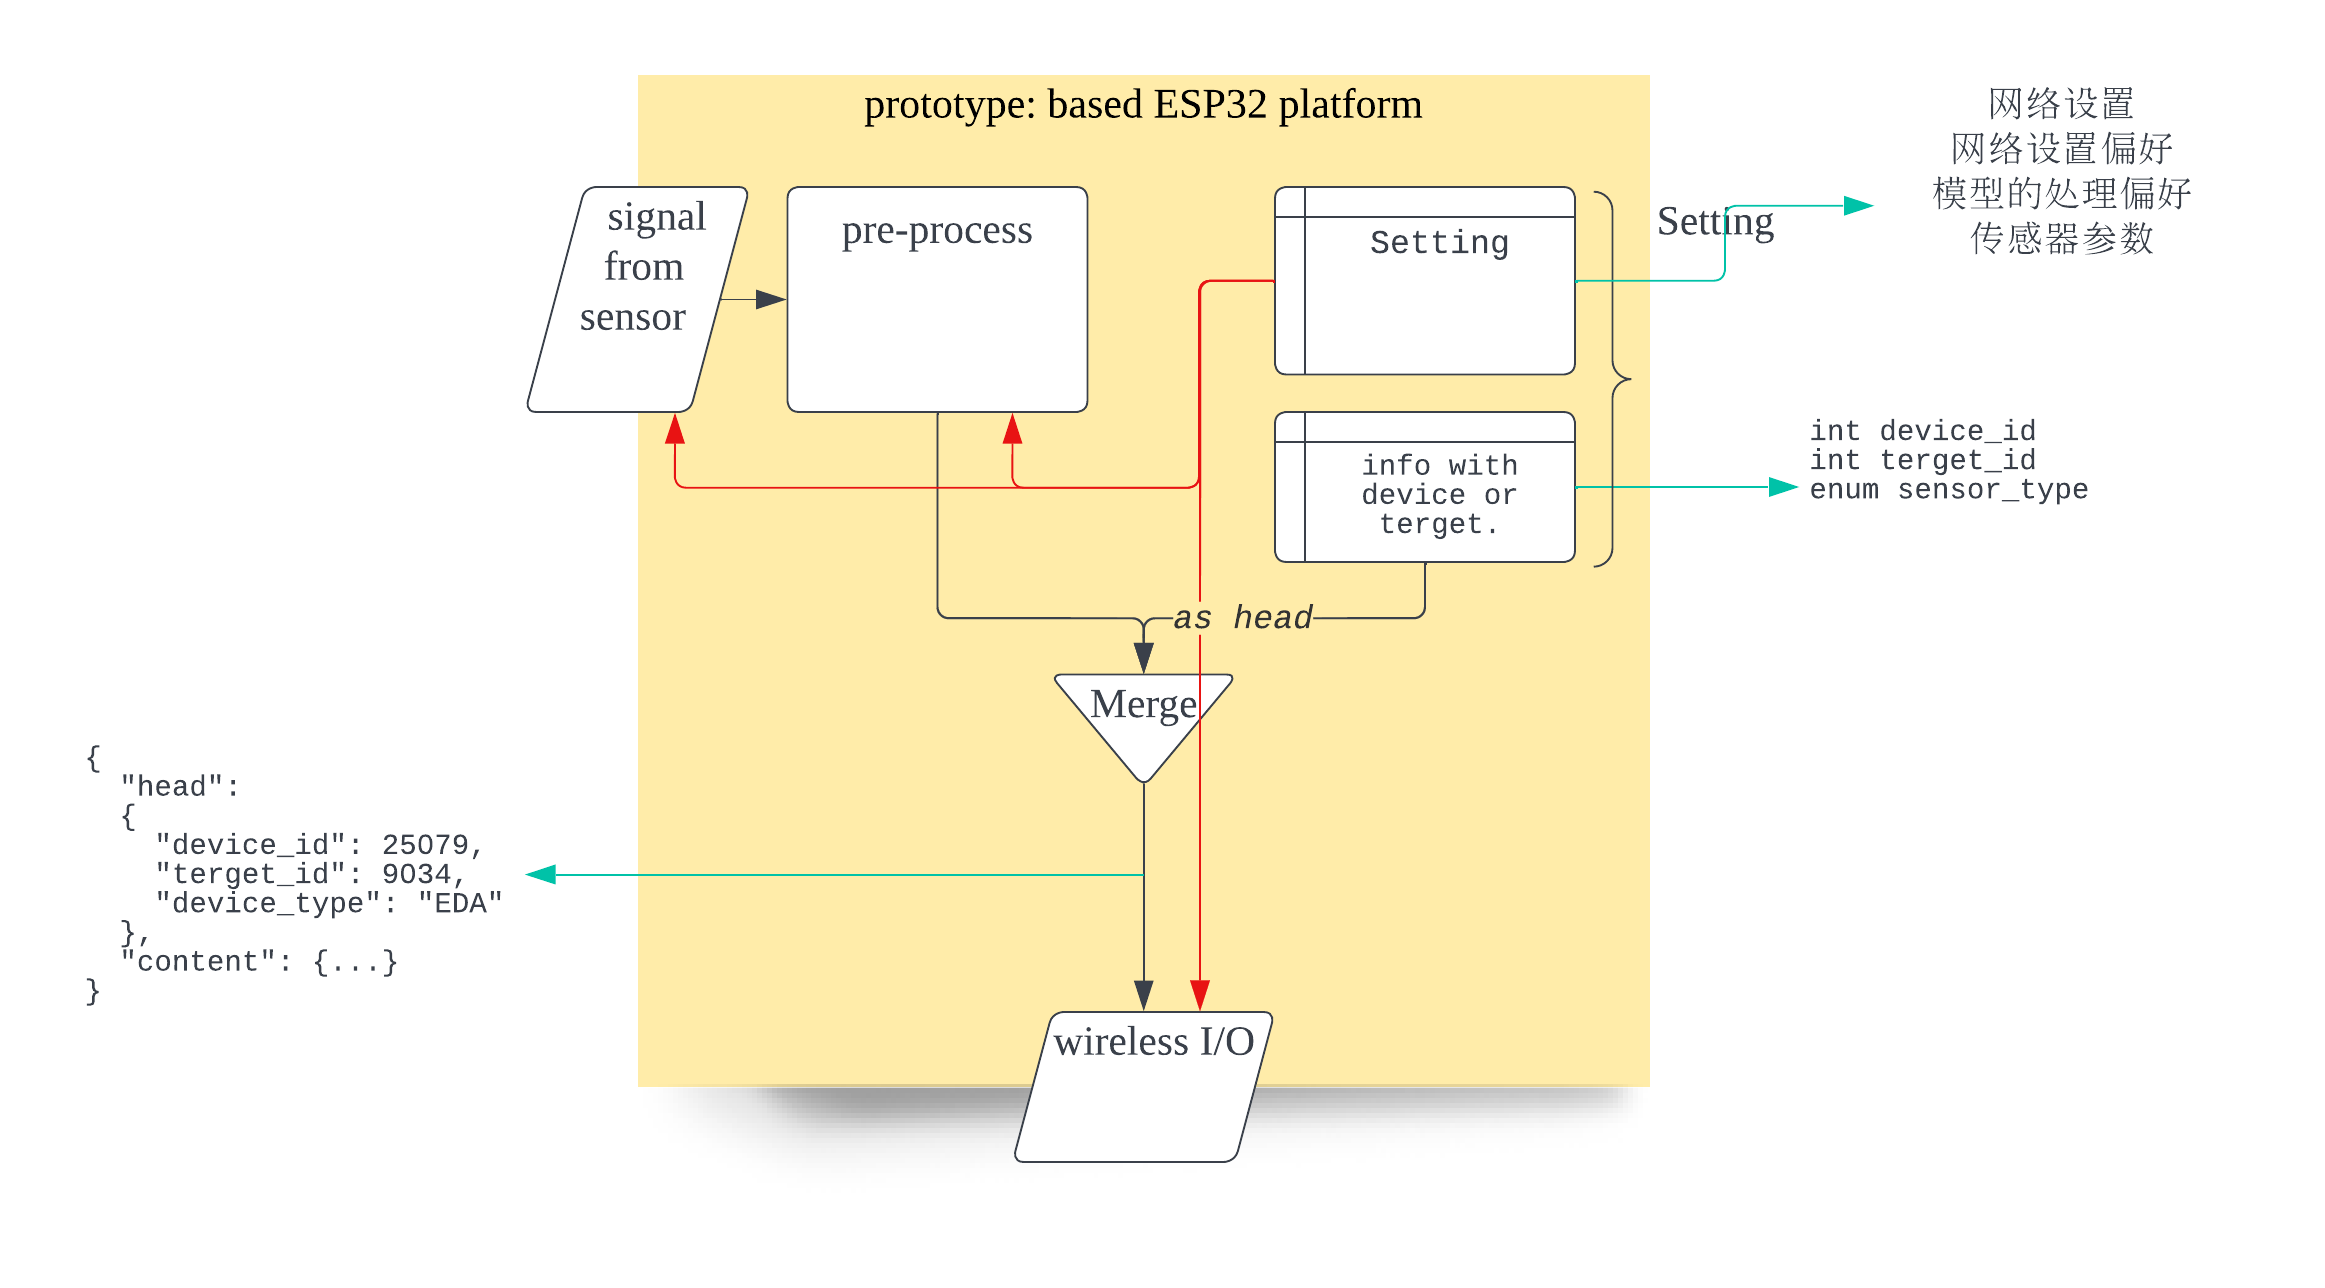
\includegraphics[width=0.95\textwidth]{Chip.png}
\centering
\caption{设备的功能框图}
\end{figure}
\par
我们在模型的构建上的思路如下,下面将花一些文本去解释:
\begin{itemize}
    \item抓取数据
    \item模型选择以及训练
    \item其他组分的构建
\end{itemize}

\subsubsection{抓取数据}

实操上可行性的分析将在这一步进行,我们将会对获得的数据进行简单分析探究该方案的可行性,同时对后期的一系列研究进行铺垫。

\begin{figure}[H]
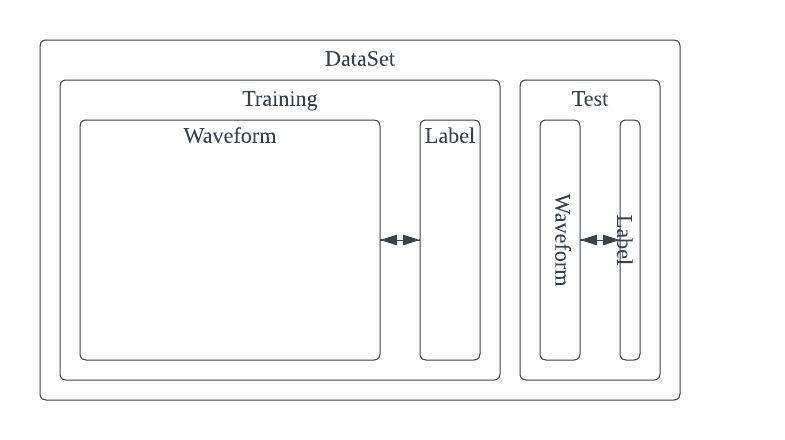
\includegraphics[width=0.75\textwidth]{ds.jpeg}
\centering
\caption{需要的数据}
\end{figure}

从时间序列中检测某种状态的概率属于机器学习范畴内的一类任务,所以需要一定量的数据用以训练。据估计可能需要几头猪数小时的生理数据以供采集。
而且为了方便判断猪的状态,可能需要同期同个体的影视资料进行辅助分析,虽然需要的内容的容量没有显著变化,
但这个工作相比于标注图片的骨骼点以及状态实在是轻松了太多。

\par
数据的格式:
\begin{itemize}
    \item波形
    \item在哪些\textbf{时间内}存在情绪波动
\end{itemize}

\subsubsection{模型选择以及训练}

我们需要将问题转化为一类机器学习的任务:
\begin{itemize}
    \item\textbf{输入}:观测得到的基于时间的电信号序列$\mathscr{O}$
    \item\textbf{输出}:下一刻/当前刻处于应激状态的\emph{概率},超过被设定的阈值将会报警
\end{itemize}

由数据的形式不难看出,我们可以使用经典的\textbf{隐马尔可夫链模型}(\emph{Hidden Markov Model, HMM})或是\textbf{循环神经网络}(\emph{RNN})来作为实现检测的载体。
而二者都已经存在了不少实现的框架或库,甚至做到了「开箱即用」的程度,所以可以经适当移植可以轻松运用以及部署。

\subsubsection{其他组分的构建}

考虑到数据的持久性以及整个项目的部署难度,我们的考虑是将后期的模型以Web服务的形式部署,并辅以简单的数据库以及简单的API接口。
\par
由于参与人员的代码水平,选择了Python作为实现服务的语言。该项目主要提供以下的功能:
\begin{itemize}
    \item封装模型
    \item将数据上传至数据库
    \item实时/接近实时的计算并返回结果
    \item提供接口以便饲养人员操作
    \item鉴权(部署在云端的情况下)
\end{itemize}

原型机的架构如下图所示:% 这部分看个乐就好

\begin{figure}[H]
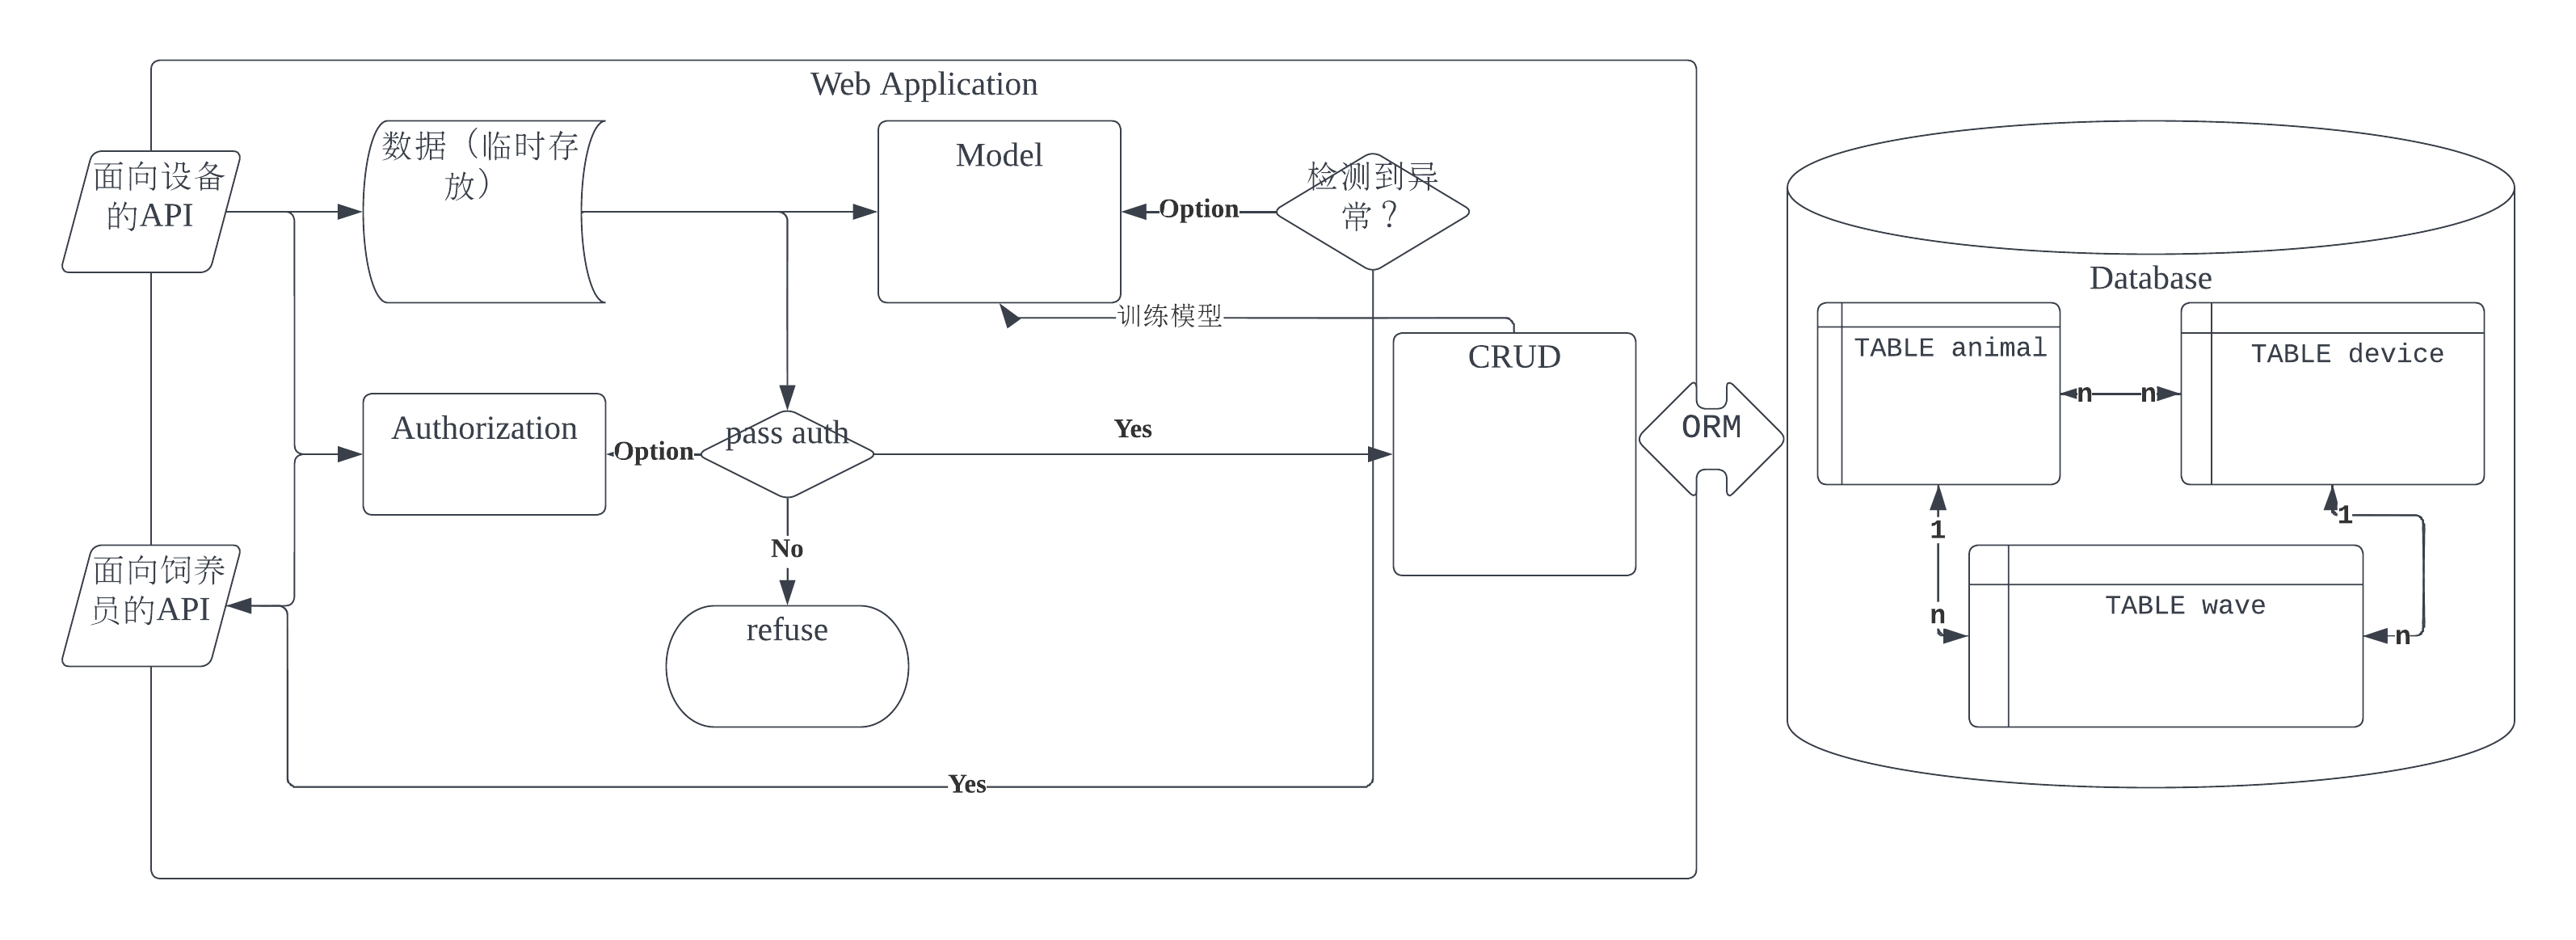
\includegraphics[width=0.95\textwidth]{WebService.png}
\centering
\caption{Web服务,生产环境下部署在局域网内。}
\end{figure}

\subsection{可行性分析}

首先是技术,如上文第 \ref{sec:31} 节引言所讲,我们选择的技术在人类中属于应用比较广泛,并且有很多文献以及研究成果对
我们思路的逻辑的完善性给予了支持。所以单从技术而言,基于生理数据的采集、处理以及分析得到动物的应激状态
或是压力水平是可行的。而之前未能得到广泛应用主要是源于缺乏廉价的设备与标准。而随着时代的发展,
设备逐渐小型化以及智能化,这为项目的落地提供了重要支持。
\par
从设备来讲,虽说已经快要到达摩根定律的所预言的极限,但是现在的电子设备的性能依旧处于健壮且相对稳定的提高期,
而深度学习的第二次寒冬结束也正是因为设备算力的大幅提高,
从另一种角度来讲,物联网的发展也带动了具有相同算力的设备也逐渐的廉价化、迷你化。
\par
愈加廉价的设备、专门设计被用于此类任务的推演设备以及物联网设备在工业界得到了广泛应用。
按照我们的估计,仅保留最基本的部分,在中小型猪场,系统甚至可以在一台树莓派上运行并提供不间断的服务。
\par
当然,从另一个角度想,哪怕难以在养殖场架设所有模型,我们也可以将服务部署在云上,
通过API来提供服务,这也可以和别的设备/参数建立联系,提高测量的准确性与鲁棒性。

\subsection{应用与价值}

考虑到成本以及环境,我们是对比较有价值的个体进行监测,例如种公猪等。
其一、种公猪需要不间断的监测而饲养员的精力有限,该系统可以部分的替代饲养员,减轻精力消耗以让其专注于更关键的任务而非维护上;
其二、应激等刺激对于种公猪的影响更大,造成的精液品质影响后果更大、经济损失更加严重,本系统的架设可以及时预警、显著的减少应激因素对猪后续潜在的刺激。
\par
我们的项目具备了比较大的商业价值以及巨大的潜力,一旦落地对于动物福利等领域将带来很大的促进作用,
并且可以能够有效的提高生产性能,可以促进产业的进一步发展。

% --- 参考文献 ---

%\newpage
\addcontentsline{toc}{subsection}{参考文献}
\bibliography{pre}% Reference \\ 4 times: LaTeX => BiBTeX => LaTeX => LaTeX

% --- 时间线 ---

\newpage
\section{时间线}
\begin{itemize}
    \item 2022-05-21 - 2022-05-31 ~传感器设计
    \item 2022-05-21 - 2022-05-26 ~模型设计
    \item 2022-06-02 - 2022-06-05 ~训练与调试
    \item 2022-05-26 - 2022-06-07 ~其他设计以及收尾
\end{itemize}

% \subsection{最新进度}

\end{document}